% Apresentação (slides) — conversão do seminario.pdf para LaTeX/Beamer.
% 21 frames (mesma contagem do seminário original).
% Conteúdo revisado: a comparação de preditores roda em CPU TIMING (em-ordem),
% conforme o tópico 2; os números seguem o relatório (main.tex) e os dados
% brutos do gem5. Teoria (branch prediction) replica o conteúdo das págs. 7-11
% de docs/seminario_atualizado.pdf.
% Compilar com: pdflatex apresentacao.tex
%   Requer o tema metropolis (TeX Live: pacote 'beamertheme-metropolis').
%   Para as fontes Fira originais, compile com xelatex ou lualatex.
\documentclass[aspectratio=169,11pt]{beamer}

\usepackage[utf8]{inputenc}
\usepackage[T1]{fontenc}
\usepackage[brazil]{babel}
\usepackage{graphicx}
\usepackage{booktabs}
\usepackage{xcolor}
\graphicspath{{figuras/}}

% --------------------------------------------------------------------
% Tema metropolis (flat / moderno) com paleta azul + coral
% --------------------------------------------------------------------
% sectionpage=none mantém os 21 slides (sem páginas-divisor automáticas)
\usetheme[progressbar=frametitle,numbering=fraction,block=fill,sectionpage=none]{metropolis}

\definecolor{primary}{HTML}{3B5B92}  % azul (barra de título)
\definecolor{accent}{HTML}{DD5E47}   % coral (progress bar / destaques)
\setbeamercolor{frametitle}{bg=primary}
\setbeamercolor{progress bar}{fg=accent}
\setbeamercolor{alerted text}{fg=accent}

\setbeamertemplate{caption}[numbered]

\title[Predição de Desvios no HeapSort]{Avaliação de predição de desvios no HeapSort em RISC-V}
\subtitle{com o simulador gem5}
\institute[UFFS]{Organização de Computadores --- UFFS}
\author{Jean C. C. Gondorek \and Jonathan G. Correa \and Kassiara R. Bosing \and Lucas S. Schuch \and Matheus H. R. da Costa}
\date{}

\begin{document}

\maketitle

% ====================================================================
\section{Introdução}

\begin{frame}{Introdução}
  \begin{itemize}
    \item No primeiro trabalho de Organização de Computadores usamos o
          simulador \textbf{Venus} para avaliar um HeapSort implementado pelo grupo.
    \item Nesta segunda etapa o mesmo algoritmo é analisado sob a ótica de
          \textbf{microarquitetura}, com o simulador de ciclo de clock \textbf{gem5}.
  \end{itemize}
\end{frame}

\begin{frame}{Introdução --- tópico escolhido}
  \begin{itemize}
    \item Tópico: \textbf{branch prediction} (predição de desvios), comparando duas técnicas:
      \begin{itemize}
        \item \textbf{LocalBP} --- preditor local simples;
        \item \textbf{BiModeBP} --- preditor global (bi-mode).
      \end{itemize}
    \item Métricas: total de desvios condicionais avaliados e número de
          predições incorretas, além de tempo e IPC.
    \item Objetivo: entender o desempenho de cada técnica em RISC-V e
          identificar qual é mais eficiente para o caso analisado.
  \end{itemize}
\end{frame}

% ====================================================================
\section{O algoritmo}

\begin{frame}{Contextualização do algoritmo}
  \begin{itemize}
    \item HeapSort implementado em assembly RISC-V no Trabalho 1.
    \item Usa um \textbf{min-heap} (árvore binária armazenada em vetor).
    \item Duas etapas: \emph{construção} do heap e \emph{extração} sucessiva dos elementos.
    \item Rotina central: \texttt{heapify}, que compara um nó com seus filhos e
          restaura a propriedade do heap.
  \end{itemize}
\end{frame}

\begin{frame}{Por que HeapSort é interessante para branch prediction?}
  \begin{itemize}
    \item \textbf{Laços regulares} (\texttt{build\_loop}, \texttt{extract\_loop}):
          padrão de desvio previsível.
    \item \textbf{Comparações dependentes dos dados} dentro de \texttt{heapify}:
          o resultado depende dos valores do vetor.
    \item O mesmo endereço de instrução pode alternar entre \emph{taken} e
          \emph{not-taken}, dificultando a predição.
  \end{itemize}
\end{frame}

\begin{frame}{Desafios de conversão do HeapSort para assembly}
  \begin{itemize}
    \item \textbf{Build do gem5}: compilação demorada ($>$2h) e inconsistente
          entre máquinas $\rightarrow$ padronização em ambiente \textbf{Docker}.
    \item \textbf{Syscalls do Venus}: pseudo-instruções didáticas substituídas por
          \texttt{printf} e \texttt{malloc} da libc.
    \item \textbf{Recompilação estática}:
          \texttt{riscv64-linux-gnu-gcc -static heapSort\_original.s -o heapSort\_original.riscv}.
  \end{itemize}
\end{frame}

% ====================================================================
\section{Fundamentação teórica}

\begin{frame}{Fundamentação teórica --- o que é branch prediction?}
  \begin{itemize}
    \item Quando encontra uma instrução condicional, o processador não sabe
          imediatamente se o salto será realizado ou não.
    \item Se esperar descobrir, o pipeline fica parado, reduzindo o desempenho.
    \item \textbf{O que é branch prediction?} É uma técnica usada em
          processadores para tentar adivinhar o resultado de uma instrução de
          desvio antes que ela seja executada.
    \item Em arquiteturas como a RISC-V, isso é importante porque o
          processador usa pipeline, evitando \emph{hazards} de controle.
  \end{itemize}
\end{frame}

\begin{frame}{Fundamentação teórica --- como funciona?}
  \begin{itemize}
    \item O preditor é consultado e, para cada branch, a CPU guarda uma
          previsão, se utilizando de padrões anteriores para definir ela:
      \begin{itemize}
        \item \textbf{Taken} (salta) $\rightarrow$ começa a buscar instruções
              do endereço \texttt{label};
        \item \textbf{Not Taken} (não salta) $\rightarrow$ continua buscando a
              próxima instrução sequencial.
      \end{itemize}
    \item Quando a condição é finalmente calculada:
      \begin{itemize}
        \item se a previsão estava correta, o pipeline continua normalmente;
        \item se estava errada, as instruções carregadas incorretamente são
              descartadas (\emph{pipeline flush}) e o processador busca as
              instruções corretas.
      \end{itemize}
  \end{itemize}
\end{frame}

\begin{frame}{Fundamentação teórica --- tipos de predição}
  \begin{columns}[t]
    \column{0.5\textwidth}
      \textbf{Estática}: sempre segue uma regra fixa sem olhar o que
      aconteceu antes
      \begin{itemize}
        \item Sempre prevê ``taken''.
        \item Sempre prevê ``not taken''.
        \item Se o salto for para trás (loop), prever Taken; se for para
              frente, prever Not Taken.
        \item É barata mas não precisa.
      \end{itemize}
    \column{0.5\textwidth}
      \textbf{Dinâmica}: aprende com as execuções anteriores e usa esse
      histórico para prever o próximo resultado
      \begin{itemize}
        \item Pode usar tabelas de bits, contadores de 2 bits, histórico
              global etc.
        \item É o método utilizado em processadores modernos.
        \item Exige mais hardware, mas é muito mais precisa.
      \end{itemize}
  \end{columns}
\end{frame}

\begin{frame}{Fundamentação teórica --- técnicas de predição analisadas: LocalBP}
  \begin{itemize}
    \item É um preditor relativamente simples que usa o histórico local de
          cada branch.
    \item Para cada instrução de desvio, mantém um histórico próprio.
    \item Observa como aquele branch se comportou nas últimas execuções.
    \item Usa esse histórico para prever a próxima execução.
    \item Boa precisão para loops e padrões repetitivos, mas requer mais
          armazenamento para guardar históricos individuais e não aproveita
          correlações entre branches diferentes.
  \end{itemize}
  \vspace{4pt}
  \textbf{Exemplo:} \texttt{beq x3, x2, label} $\rightarrow$ \texttt{TTTNTTTN} \\
  O preditor aprende que esse branch geralmente é tomado e ajusta sua
  previsão de acordo.
\end{frame}

\begin{frame}{Fundamentação teórica --- BiModeBP}
  \begin{itemize}
    \item Preditor mais sofisticado, criado para reduzir interferências entre
          branches com comportamentos opostos.
    \item Possui tabelas especializadas para branches que tendem a ser
          \emph{taken}, branches que tendem a ser \emph{not taken}, e uma
          tabela de escolha que decide qual das duas consultar.
    \item Possui muito mais previsibilidade e menos interferência entre
          branches, mas o consumo de hardware é bem maior.
  \end{itemize}
  \vspace{4pt}
  \textbf{Exemplo:} Branch A quase sempre \emph{Taken}; Branch B quase sempre
  \emph{Not Taken}. Em um preditor simples, ambos podem disputar as mesmas
  entradas da tabela e prejudicar a precisão. O BiMode separa esses
  comportamentos, reduzindo esse efeito, conhecido como \emph{aliasing}.
\end{frame}

% ====================================================================
\section{Metodologia}

\begin{frame}{Metodologia --- adaptação do código}
  \begin{itemize}
    \item Assembly adaptado do Venus para o gem5: sintaxe GCC, ponto de entrada
          \texttt{main}, \texttt{printf}/\texttt{malloc}, binário RISC-V estático.
    \item Lógica preservada: \texttt{heapSort}, \texttt{heapify}, \texttt{swap}.
    \item Variou-se a frequência de clock (2, 3 e 4 GHz) para observar o impacto
          no tempo total de simulação.
  \end{itemize}
\end{frame}

\begin{frame}{Metodologia --- cenários comparados}
  \begin{itemize}
    \item Dois cenários, demais parâmetros de hardware \textbf{fixos}:
      \begin{itemize}
        \item \textbf{Cenário A} --- LocalBP (preditor local simples);
        \item \textbf{Cenário B} --- BiModeBP (bi-mode global).
      \end{itemize}
    \item Entrada padrão: $n = 6$ (\{12, 11, 13, 5, 6, 7\}).
    \item Benchmark complementar: $n = 100.000$ para validar em escala.
  \end{itemize}
\end{frame}

\begin{frame}{Metodologia --- métricas coletadas}
  Extraídas de \texttt{m5out/stats.json} após cada simulação:
  \begin{itemize}
    \item \texttt{branchPred.BTBLookups} --- total de desvios avaliados;
    \item \texttt{branchPred.condIncorrect} --- predições incorretas;
    \item \texttt{simTicks} --- tempo total de simulação;
    \item \textbf{IPC} = \texttt{simInsts / core\_numCycles}.
  \end{itemize}
  \vfill
  Taxa de erro global = \texttt{condIncorrect / committed}
  (predições incorretas sobre desvios commitados).
\end{frame}

\begin{frame}{Metodologia --- configuração experimental}
  \begin{columns}[t]
    \column{0.5\textwidth}
      \textbf{Comparação de preditores}
      \begin{itemize}
        \item CPU \textbf{TIMING} (pipeline em-ordem)
        \item LocalBP vs. BiModeBP
        \item Demais parâmetros fixos no par
      \end{itemize}
    \column{0.5\textwidth}
      \textbf{Escalas testadas}
      \begin{itemize}
        \item $n=6$ (entrega parcial)
        \item $n=100.000$ (validação em escala)
        \item Clock 3 GHz; L1 32 kB; L2 256 kB
      \end{itemize}
  \end{columns}
  \vfill
  \footnotesize\textit{Observação: na CPU em-ordem (TIMING) a troca de preditor
  não altera o \texttt{simTicks} --- esse modelo não penaliza ciclos por
  \emph{misprediction}; por isso o ganho do BiModeBP aparece na contagem de
  erros, não no tempo simulado.}
\end{frame}

% ====================================================================
\section{Resultados}

\begin{frame}{Resultados --- erros de predição ($n=6$, pipeline em-ordem)}
  \centering
  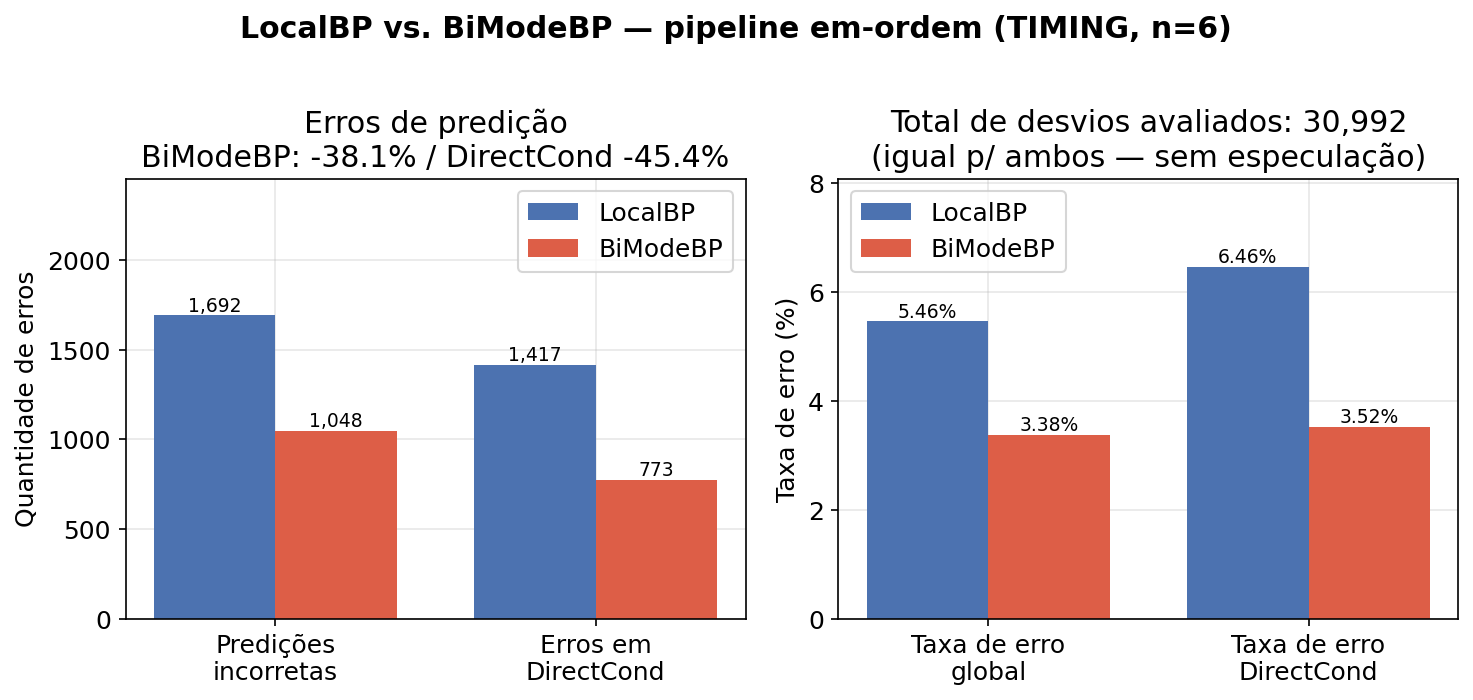
\includegraphics[width=0.9\textwidth]{comparacao_inorder.png}
  \par\smallskip\small O total de desvios avaliados é idêntico (30.992) ---
  o BiModeBP reduz as predições incorretas em $\sim$38\%, concentrado nos
  desvios condicionais diretos (\texttt{DirectCond}) de \texttt{heapify}.
\end{frame}

\begin{frame}{Resultados --- por que o tempo não muda?}
  \begin{itemize}
    \item O pipeline \textbf{em-ordem (TIMING)} mede corretamente \emph{quantos}
          erros de predição ocorrem.
    \item Porém esse modelo \textbf{não aplica penalidade de ciclos} por
          \emph{misprediction} --- não há \emph{flush} especulativo a custar tempo.
    \item Por isso o \texttt{simTicks} é \textbf{idêntico} entre LocalBP e
          BiModeBP, mesmo com 38\% menos erros.
    \item O ganho do BiModeBP, neste modelo, é de \textbf{precisão}, não de
          tempo de execução simulado.
  \end{itemize}
\end{frame}

\begin{frame}{Resultados --- tabela comparativa ($n=6$, CPU TIMING)}
  \centering
  \begin{tabular}{lrrr}
    \toprule
    \textbf{Métrica} & \textbf{LocalBP} & \textbf{BiModeBP} & \textbf{Var.} \\
    \midrule
    Desvios avaliados (lookups) & 30.992 & 30.992 & 0\% \\
    Predições incorretas        & 1.692  & 1.048  & $-$38,1\% \\
    Taxa de erro global         & 5,46\% & 3,38\% & $-$2,08 p.p. \\
    Erros em DirectCond         & 1.417  & 773    & $-$45,4\% \\
    Taxa de erro DirectCond     & 6,46\% & 3,52\% & $-$2,94 p.p. \\
    \texttt{simTicks}           & \multicolumn{2}{c}{106{,}6\,M (idêntico)} & 0\% \\
    \bottomrule
  \end{tabular}
\end{frame}

\begin{frame}{Resultados --- efeito de escala}
  \centering
  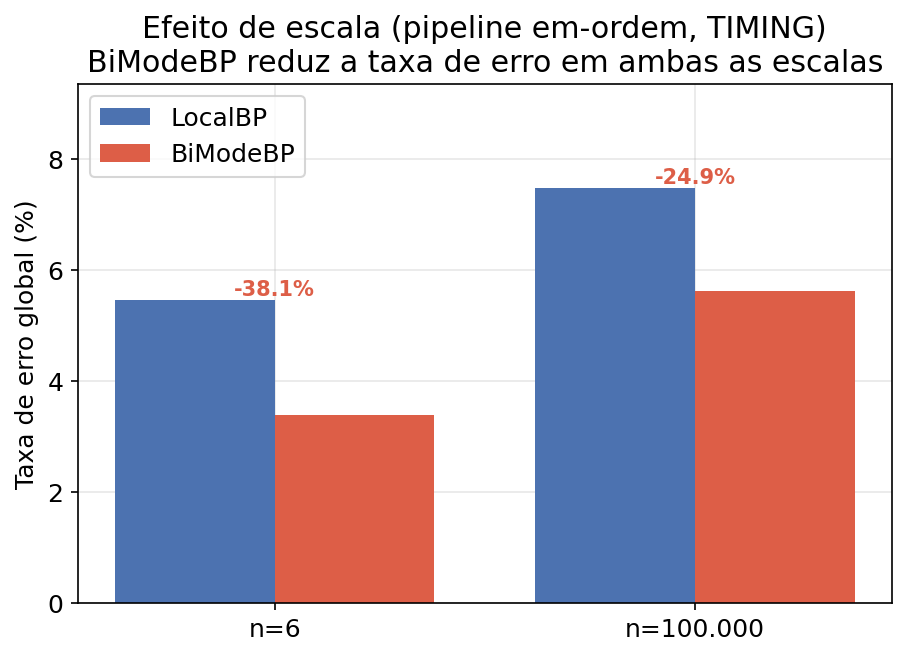
\includegraphics[width=0.75\textwidth]{efeito_escala.png}
  \par\smallskip\small Em $n=100.000$ o BiModeBP reduz a taxa de erro em
  24,9\% (vs.\ 38,1\% em $n=6$); o \texttt{simTicks} permanece idêntico entre
  preditores em ambas as escalas --- o modelo em-ordem não penaliza ciclos por
  \emph{misprediction}.
\end{frame}

% ====================================================================
\section{Conclusão}

\begin{frame}{Conclusão}
  Para o HeapSort em RISC-V no gem5, em pipeline \textbf{em-ordem (TIMING)}, o
  \textbf{BiModeBP} adapta-se melhor que o \textbf{LocalBP}:
  \begin{itemize}
    \item Redução de $\sim$38\% nas predições incorretas ($n=6$), mantida em
          escala (24,9\% em $n=100.000$);
    \item Ganho concentrado nos desvios dependentes de dados de \texttt{heapify},
          onde o mesmo PC alterna entre taken/not-taken a cada recursão;
    \item O \texttt{simTicks} é idêntico entre preditores --- o modelo
          em-ordem não penaliza ciclos por \emph{misprediction}: o ganho do
          BiModeBP é de \textbf{precisão}, não de tempo simulado.
  \end{itemize}
\end{frame}

\begin{frame}{Conclusão --- recomendação}
  \begin{itemize}
    \item Os laços regulares (\texttt{build\_loop}, \texttt{extract\_loop}) são bem
          servidos por ambos os preditores; a diferença real aparece no \texttt{heapify}.
    \item \textbf{Recomendação}: o BiModeBP é preferível para cargas com mistura de
          laços regulares e comparações dependentes de dados, como o HeapSort.
    \item \textbf{Trabalho futuro}: repetir a comparação em pipeline fora de
          ordem para observar o efeito da predição sobre o tempo de execução.
  \end{itemize}
\end{frame}

\end{document}
